\documentclass[11pt]{report}
\usepackage[a4paper]{geometry}
\usepackage{amsmath}
\usepackage{amsfonts}
\usepackage{mathabx}
\usepackage{amsthm}
\usepackage{amssymb}
\usepackage{framed}
\usepackage{relsize}
\usepackage{subfig}
\usepackage{graphicx}
\graphicspath{ {images/}}
\usepackage{subcaption}
\usepackage{enumerate}
\usepackage{booktabs}
\usepackage{csquotes}

\usepackage[
authordate,
maxcitenames=1,
backend=biber,
natbib,
maxbibnames=6
]{biblatex-chicago}
\addbibresource{project.bib}
\bibliography{project}

\usepackage[usenames,dvipsnames]{xcolor}
\usepackage{tikz}
\usetikzlibrary{arrows}

\usepackage{listings}
\usepackage{minted}
\lstset{language=Python, breaklines=true, basicstyle=\footnotesize}  
\usepackage{fancyhdr}
\setlength{\parindent}{0pt}
\pagestyle{fancy}
\fancyhf{}
\fancyhead[R]{Michael Redman, CID:\ 00826863}
\fancyfoot[C]{\thepage}
\begin{document}
\title{Detecting pathologies in spatiotemporal data}
\author{Michael Redman, CID:\ 0082686\textbf{3} \\%
Supervised by Professor Axel Gandy\\
M4R}
\date{June 2017}

\maketitle

\begin{abstract}
In this project, we examine the application of spatiotemporal models on epidemiological data. Through the use of both descriptive and generative models, we seek to identify abnormal patterns in a set of simulated data and compare and contrast the different models accuracy and computational cost. We suggest a novel description of the `in-control' rate for a cumulative sum control chart and improve on the efficiency of two existing Bayesian models in the literature.
\end{abstract}

\renewcommand{\abstractname}{Acknowledgements}
\begin{abstract}
In addition to my advisor, Professor Axel Gandy, I would like to thank Dr. Marta Blangiardo for her invaluable advice and guidance throughout the project and Dr Fred Piel \& Areti Boulieri for their helpful and supportive conversations.
\end{abstract}

\tableofcontents

\chapter{Introduction}

The identification of unusual patterns of disease is of obvious importance in public health. Discrepencies in the relative risk of disease incidence between regions will both inform the allocation of medical resources and motivate investigations over possible environmental exposure. \\

 The detection of such discrepencies is often done by the use of disease mapping studies which aggregate the recorded incidents of the disease of interest over time, and compare the total counts between regions. Public health information systems now record this data indexed to such a fine degree of granularity that the detection of risk factors which act at a very local level, such as hazardous industrial waste, can be feasably indentified. However this fine-grained approach will leave the examined regions with very low incidence, which can hinder the isolation of the signal from the noise, hence the use of time aggregated values. However, in doing this we relinquish any potential information that a temporal trend may afford us. In fact, as described in \citet{stability}, the nature of the temporal trend may suggest anomalities related to very different kinds risk factors. A region which conforms to a similar temporal trend as the others---for example a seasonal factor---but at a higher rate would imply a disparity which acts over the whole time period, such as an enviromental issue or a sociodemographic difference. While a region which acts wildly without regard to the general trend might suggest a more acute issue is at play. \\

Consequently, in this project we will be looking at data that is indexed in both space and time. Additionally in any model that we implement, we wish to be able to control for known covariates which may influence the risk within a given region. For example some regions will be more populous, while others may contain proportionally more at-risk peoples, so it would be wise to have some method of setting the expected counts by region. \\

A variety of methods have been investigated in these contexts. One of the most simple is that of scan statistics. This procedure, implemented in software such as SaTScan, seeks to identify clusters which can not be explained by the base process -- in our case typically an inhomogenous Poisson process. It does this by evaluating all possible ``windows'' in turn, where a given window will include the region in question and its ``neighbours'' both spatially and temporally. This forms a kind of cylinder which acts to smooth the observed counts in space and time, allowing the sparse data as described earlier to be examined without the noise overwhelming any underlying spatial heterogenicity. This method is descibed in detail and applied to epidemiological data in \citet{scan}. While offering an improvement over pointwise evaluation, spatial scan statistics by nature of this smoothing construction are limited in their ability to detect abnormalities at the individual level, i.e. isolated to a particular region \citep{baystdetect}.  \\

Control chart based methods offer both relatively fast computation times and the ability to specifically identify abnormal temporal trends. These, in the simplest of terms, are graphs we construct combined with a decision rule to classify whether a process is in `in-control' or `out-of-control'. Versions such as CUSUM are often designed for step detection -- the identification of abrupt jumps in rate of the process. When looking at longer time periods, this is exactly the type of pathology one might expect. The regions which now show atypical trends should still have exhibited normal behaviour most of the time, the problem is to decide when such heterogeneity in the process is substantive.  Another advantage is, as the techinique is sequential in nature, the sample size of the items in consideration need not be fixed in advance.  \\

The most natural way to frame our problem is by the construction of a hierachical model. In this method we perform inference on a latent variable---within a complex model---which indicates the `unusalness' of a point or group of points. This Bayesian approach compells us to express our assumptions about the data generatively, which confers a number of advantages. Firstly, it is often the case in discriminative models that the choice of method is implicitly performing shrinkage, without this being made explicit or even realized by the modeler. For an intereting example see \citet{stoch}. Thinking generatively forces us to be clear about our assumptions. Secondly, real world epidemiological data will presumably not supply the true response variable, that is, whether or not a region is genuinely anomalous. This abscence of training means we need our model to provide reasonable estimates immediately, rather than at some asymptotic limit. This advantage can be seen in, for example, \citet{ng}. Thirdly, the parameters of a Bayesian model are far more readily interpretable that those in a non-generative setting, which could allow for further inference beyond the identification of abnormal regions, e.g. the nature and extent of the deviation from what was expected. And lastly,
 the Bayesian framework naturally allows the addition of futher assumptions and complexity. For example, \citet{banerjee} extends spatiotemporal models to the modelling of multiple diseases via the introduction of a shared `frailty' term. \\

The examination, implementation and comparison of these Bayesian methods with discriminative models, specifically control charts, is the focus of this project. \\

Working on simulated data, we first implement a CUSUM based classifier and suggest a novel specification of the `in-control' process. With the efficiency of the method being of great importance, we implement the computations from scratch in Fortran rather than modifying the existing statistical routines in R. \\

Then, turning to Bayesian methods, we examine the general structure of the models employed in the literature and how this standard is well suited to the particular challenges of our problem. In particular, the favored priors for the smoothing of the data are reviewed. The difficulties and subtleties of computaion are addressed in detail, as are some of the superior techniques that have been developed in the past few years. \\

We examine BaySTDetect, one of the existing models in the literature, discussing the rationales behind the construction of the model and the `cutting of feedback' that is employed -- where we demonstrate that this particular choice is fundamental to its success. Rather than use the standard MCMC software in the field, we implement the model in Stan using Hamiltonial Monte Carlo and combine the submodels directly through the likelihoods. We show that this can lead to order of magnitude speed-ups over the original implementation in \citet{baystdetect}. \\

We then suggest a new model, based on \citet{stability}, that works fully within the Bayesian framework by identifying an excess in the variance which can not be explained by the shared random effects. Implementing this model, again in Stan, we show that this model obtains good results, despite not being the way in which our simulated data were originally created. However, as suggested in \citet{best2005comparison}, models of this kind may oversmooth the counts spatially. We demonstrate this by simulating a new set of data where the regions to be `unusual' are selected sequentially via a preferential attachment scheme and showing that our model performs poorly in this context. \\

Finally we compare the use three models on both sets of data with respect to their speed, false postive rate and power.

\chapter{Simulated data}

In order to test the accuracy of any potential models we need some data that exhibits the type of pathological trends that we wish to identify. The data used in this project that we describe here was graciously supplied by Areti Boulieri.

\section{Specification}

A real dataset of asthma hospitalisation counts was used to contruct the expected rates, adjusted by regional demographics by age and sex, for the 221 Clinical Commisioning Groups in England. These are the expected counts that we will standardize against when attempting to identify abnormalities. We denote these values throughout by $E_{i}, \text{ for } i=1,\ldots,221$. A plot that we generated to show the distribution of these values across the regions can be seen in fig \ref{fig:mapped} (a). \\

A binomial random variable might be the most principled choice of response but the expected counts we have calculated are large enough for using a Poisson response to be essentially equivalent. Indeed this is the most popular choice in the literature. The data was generated across 15 time points, so our values are drawn from
\begin{equation}
Y_{i,t} \; \sim \; \operatorname{Poisson}(E_i \cdot \mu_{i,t}), \ \ \ \ i=1,\ldots,221 \ \ \ \ t=1,\ldots,15
\end{equation}

where $\mu_{i,t}$ allows us to add random effects to our model. \\

These random effects are used to add additional natural variation to the counts, where the direction of this variation is in some sense shared between `similar' regions or time points. We seperate these effects into those that describe the temporal trend and those which affect the spatial heterogeneity. So for the temporal trend we of course expect adjacent time points to be similar. This is achieved in this data by sampling from a one-dimensional Gaussian random walk
\begin{equation}
\xi_{1:15} \; \sim \; \operatorname{RW}_1(\sigma_{\xi}^2).
\end{equation}

Additionally, we would expect regions which are close to each other to be similar. The data generation incorporated this assumption by the use of the BYM prior, first defined in \citet{bym},
\begin{equation}
\lambda_{1:211} \; \sim \; \operatorname{BYM}(W, \sigma_{\lambda}^2, \sigma_v^2) 
\end{equation}
which is a multivariate normal distribution
\begin{equation}
\lambda_{1:211} \; \sim \; \mathcal{N}(v_{1:211}, I_{211} \cdot\sigma_{\lambda}^2)
\end{equation} 
where the mean vector is drawn from an \emph{intrinsically autoregressive} process
\begin{equation}
v_{1:211} \; \sim \; \operatorname{IAR}(W, \sigma_v^2)
\end{equation}
which is a Markov random field where areas that are adjacent (according to an adjacency matrix $W$) are more similar to those further away. The precise specification of the BYM prior is discussed in section \ref{carmodel}. \\

The presumed sources of these random effects will determine how we wish for them to influence the generation of the data. In this dataset it is assumed that the temporal and spatial effects will work multiplicatively, where increases in one will magnify the effect of the other. Therefore, given our samples from the aformentioned distributions, we calculate $\mu_{i,t}$ additively on the $\log$ scale
\begin{equation}
\log{(\mu_{i,t})} = \lambda_i + \xi_t \ \ \ \ i=1,\ldots,221 \ \ \ \ t=1,\ldots,15
\end{equation}

In total, this scheme describes a method of generating random variables that has the features one would expect of spatiotemporal disease incidence. We now need to modify a selection of the regions to resemble a regions we would expect to be unusual. \\

Fifteen of the regions were chosen according to the 10th, 25th, 50th, 75th and 90th percentiles of the median expected counts over time, with three regions per percentile. At each percentile the three regions were selected corresponding to one of three levels of spatial risk, i.e. the generated spatial effect $\lambda_{1:211}$, low (10th-30th percentiles), medium (45th-55th percentile) and high (70th-90th percentiles). This was done to ensure that the unusual regions were spread evenly given the underlying levels of risk. \\

To make these regions unusual they were given a deviant temporal trend. This was done by modifying the temporal trends of these regions manually, where---writing the original trend as $g(t)$ and the modified trend as $g^*(t)$---we have:
\begin{align}
g^*(t) &= g(t) + \log(2) && t = 1, 10, 11 \\ 
g^*(t) &= g(t) - \log(2) && t = 5, 15
\end{align}

This has the effect of either doubling or halving the expected counts depending on the time point. The resulting temporal trend compared to the original can be seen in figure \ref{fig:timeeffects}. \\

 N.B. All of the unusual regions exhibit the same deviation, which is probably an unrealistic assumption. However, by the way that they're defined, it is clear that the models used in this project should not perform better because of this fact. 

\begin{figure}
\includegraphics[scale=0.5]{plot_time_effects}
\centering
\caption{The general and abnormal temporal trends of the generated data. Created by Areti Boulieri}
\label{fig:timeeffects}
\end{figure}

\section{Cleaning and wrangling}

Of the 211 regions only one had no neighbours, the Isle of Wight. As this will complicate some of the smoothing calculations we need to perform for the Bayesian procedures (and the Isle of Wight was not one of those selected as unusual), the region was removed to simplify calculations.

Shape data for the 211 Clinical Commisioning Groups plus wales was provided by the SAHSU. The regions of Wales and the Isle of Wight were of course removed. The shapefiles were imported and edited using the package \emph{rgdal} created by \citet{shaperead}. Then, using the package \emph{spdep} created by \citet{shape}, the shapefile was used to generate an object which calculates all of the adjacent regions for each region. Then this object was converted into into an adjacency matrix $W$ such that
\begin{equation*}
{(W)}_{ij} &= 
\begin{cases}
1, \ \ i \leftrightarrow j \\
0, \ \ \textrm{otherwise}
\end{cases}
\end{equation*}
where the double arrow signifies adjacency. The result of this procedure can be seen over the original shapedata in fig \ref{fig:mapped} (b).


\begin{figure}
\centering
\subfloat[Expected]{\includegraphics[width=0.5\textwidth]{expected}} \label{fig:expected}
\subfloat[Adjacency]{\includegraphics[width=0.5\textwidth]{adjacency}} \label{fig:adjacency}
\caption{Mapped data}
\label{fig:mapped}
\end{figure}

\chapter{Control charts}


The use of control charts are widespead in the area of statistical quality control and have recently increasingly found use in fields such as epidemiology, see for example \citet{mei}. Their relative simplicity and ease of computation compared to most other methods makes them an ideal model to compare against, in order to observe any gains we might obtain from more complex modelling. Indeed, as expressed by \citet{vapnik} in the context of generative vs discriminative models, ``one should solve the problem directly and never solve a more general problem as an intermediate step''. \\

\section{CUSUM}

We will specifically be looking at the use of CUSUM models, which seek to identify a qualitative change in the nature of a time series via the evaluation of the cumulative sum of a relavant test statistic. In the setting of the inhomogenous Poisson CUSUM, we assume that the data follows a null model defined by a series of rate parameters which define the `in-control' Poisson process. Likewise we have a complementary set of parameters that define the rates of an `out-of-control' process. We wish to detect the point in time at which there is sufficient evidence that the process has switched from the null to the `out-of-control' process, as quickly as possible while not exceeding some measure of how often we err. \\

To do this, define $S_t$ as the value of the control chart at time $t$ and progress its value as follows
\begin{gather}
S_0 = 0 \\
S_{t+1} = \max{(0, S_t + K_{t+1})}.
\end{gather}
where $K_t$ is the value of a statistic calculated at time point $t$. \\

As first proposed in \citet{page}, we will use
\begin{align}
K_t &= \log{\left(\frac{f_1(Y_{i,t})}{f_0(Y_{i,t})}\right)} \\
    &= \log{[f_1(Y_{i,t})]} - \log{[f_0(Y_{i,t})]}.
\end{align}
where $f_0$ is the likelihood of the `in-control' rate and $f_1$ that of the `out-of-control'. \\

That is, the $\log$ of the ratio between the likelihoods of the data, at the time point, under the `in-control' and `out-of-control' Poisson process. So if likelihood of the `out-of-control' rate is greater than the `in-control' then the value of $S_t$ will increase and vice-versa. We then signal that the process is pathological if the value of $S_t$ exceeds some threshold value $h$. \\

Note that, for a Poisson process, the likelihood is
\begin{equation}
f_j(x) = \frac{\lambda_j^x e^{-\lambda}}{x!}.
\end{equation}
So for the log-likelihood we have
\begin{equation}
\ell_j(x) = x \log(\lambda_j) - \lambda_j - \log(x!)
\end{equation}
giving the value of our test statistic as
\begin{equation}
K_t = Y_{i,t} (\log{\lambda_{1, t}} - \log{\lambda_{0, t}}) - (\lambda_{1, t} - \lambda_{0, t}).
\end{equation}

This leaves us to come up with sensible methods of generating the `in-control' and `out-of-control' rates and the threshold value that we trigger at. With the data that we are examining in this project we have the expected values of the disease rates in each region and could use these for the values of the `in-control' rate but this would neglect the fact that we expect the incident counts at each region to vary over time and---importantly---this is not neccasarily pathological behaviour. It is instead a temporal trend which differs from some general (here country-wide) trend which we wish to detect. Therefore the method we propose here is to construct a general temporal trend from an average across the regions and to weight this trend per region by that regions expected counts. \\

So for the data $Y_{i,t}, \ i = 1, \ldots, R, \ t = 1, \ldots, T$ we normalize the temporal pattern of each regions by its expect count $E_{i}$ as follows
\begin{equation}
\tilde{Y}_{i, t} = \frac{Y_{i, t}}{E_{i}}, \ \ \ \ i = 1, \ldots, R, \ t = 1, \ldots, T.
\end{equation} 

We then construct the `in-control' rate for each region $I_{i, t}$ as described
\begin{equation}
I_{i, t} = E_i \cdot \frac{1}{R} \sum_{i=1}^R \tilde{Y}_{i, t}, \ \ \ \ i = 1, \ldots, R, \ t = 1, \ldots, T.
\end{equation}

For simplicity we only consider the case of abnormally high count rates and ignore artificially low counts although this could be incorporated into the CUSUM model if desired. So to define the `out-of-control' rate it makes sense to follow the same temporal trend but with a modified general rate. We do this by calculating the `out-of-control' rate $O_{i,t}$ as a multiple of the `in-control' as follows
\begin{equation}
O_{i,t} = \alpha \cdot I_{i,t}, \ \ \ \  i = 1, \ldots, R, \ t = 1, \ldots, T.
\end{equation} 
with $\alpha > 1$. \\

Now for a given value of $\alpha$ we need a threshold level at which to signal. This can be done by calculating the average-run length (ARL) which is the expected length of the series between flags of the model. The ARL on the `in-control' rate will then give a measure of the false positives for a given threshold $h$, which we can optimize with respect to. As the length of the series we are examining is fixed and the calculation of an ARL would not be clearly defined for a series of varying expectation we will not use the ARL metric here. Instead we simply simulate the `in-control' sequence for each region a large number of times and find the smallest value of $h$ for which the the false-postive rate is below some desired rate. \\

The setup as described was implemented as a Python class acting as a wrapper to a series of subroutines in Fortran via F2PY\footnote{I originally wrote the entire process in Python but the calculation of the $h$ values was far too slow to be practical. The original code can be on my Github.}. The code can be found in the appendix. \\

This CUSUM process was applied to the asthma data with the ratio $\alpha$ set to $1.5$, indicating we consider the `out-of-control' rate to be 50\% greater than the `in-control', with each regions temporal pattern being simulated 10,000 times to determine the optimal threshold values. This identified 25 regions as `out-of-control' out of the total 210, giving a false-negative rate of 0\% and false-positive rate of 5.13\%. \\

The power of the test is excellent, but the false-positive rate is clearly much greater than our desired limit of 1\%. Why is this? \\  

Note that the expected value of $K_t$ under the `out-of-control' model ($H_1$) will be the Kullback-Leibler divergence between the two models \citep{weighed},
\begin{align*}
\mathbb{E}[K_t | H_1] &= \int_{-\infty}^{\infty} f_1(x_t) K_t \; dx_t \\
                        &= \int_{-\infty}^{\infty} f_1(x_t) \log{\left(\frac{f_1(x_t)}{f_0(x_t)}\right)} \; dx_t \\
                        &= D_{\mathrm{KL}}(H_1\|H_0).
\end{align*}

This gives an intuitive explanation of the procedure: under the alternate (`out-of-control') model, $K_t$ measures the information lost by attempting to approximate the (true) alternate model by the null. When the cumulative information lost by this approximation becomes intolerable, we reject the null. \\

It can be shown that, under some assumptions, using this metric with the CUSUM method is in some sense optimal \citep{ritov1990}. However, the issues with the assumptions here are clear. The null model as we have defined attempts to incorporate the general temporal trend but we would also expect a level of random spaital variation which masks the underlying abnormalities and our procedure ignores this. Therefore for regions which are not unusual (call these $H_G$), the null model will underestimate the likelihood of their counts relative to the true likelihood. So, under $H_G$ one would expect $\log(f_1(x_t)) - \log(f_0(x_t))$ to be large more often than under the null, underestimating the value of $h$ which would be required to keep the FPR under 1\%. \\

Additionally, even if the true data is distributed as we assume in the null, the parameters of the temporal trend that defines the `in-control' models are still an estimation from the data. The errors between this hypothetical `true' temporal trend and our estimate from the data will add additional noise into the process. In particular, this will affect the estimation of the optimal value of $h$ for a given FPR -- potentially increasing the number of false positives relative to what we might otherwise expect. \\

A number of methods exist that attempt to account for this additional estimation error. For example, following the method devised in \citet{gandy}, we could estimate the `in-control' parameters as usual and then draw samples with replacement from the `in-control' model with these parameters. Then, calculating estimates of the `in-control' rates from these samples, we obtain a series of bootstrap estimators. The optimal values of $h$ for each of these bootstrap estimators can be used to devise a threshold which posseses our desired properties with a certain probability. Of course, the data from which we estimate the temporal trend is not all `in-control', so our estimates will be even more biased than this would suggest. 
 
\section{Spatial CUSUM}

While our method accounts for a varying temporal trend, it falls short most saliently by not accounting for the spatial effects we assume our data posseses. The approach suggested by \citet{raubertas} attempts to take the spatial information into account by replacing the counts at each region by a weighted sum
\begin{equation*}
x_{i,t}' = \sum_{j=1}^R s_{i, j} x_{j, t}
\end{equation*} 
where we pool within neighbourhoods by assigning the weights based on the `closeness' of the regions. \\

For example this method was used in \citet{spatialcusum} with the Poisson CUSUM, where the counts at each region were replaced by
\begin{equation*}
x_{i,t}' = \sum_{x_{j, t} \in \partial x_{i,t}} x_{j, t} 
\end{equation*} 
where $\partial x_{i,t}$ are all the regions including and adjacent to $x_{i,t}$. \\

The Poisson CUSUM statistics were calculated for these modified regions and the Benjamin-Hochberg procedure was used to determine the level at which we signal for a given false discovery rate. Despite this methods simplicity, the author uses a set of simulated data to show that it can provide a significant improvement on considering the regions individually. \\ 

This approach could be used in conjunction with that of the previous section to account for both spatial and temporal effects, while still enjoying the benefits of CUSUM. Note that, in this case, the expected counts would also need to be summed across neighbourhoods to provide the `in-control' means. 

\chapter{The Bayesian Framework}

A sensible way of improving on this would be to use a generative model which incorporates both a flexibility that describes our uncertainty around the parameterization of the model and makes explicit our beliefs as to the structure of the data. This is most naturally done in the Bayesian framework, where we specify the model in terms of a likelihood which describes how we simulate the data based on a set of parameters and a collection of---possibly hierarchical---priors which describe our uncertainty about these parameters ex ante. \\

The evaluation of the posterior from this description is then given by Bayes formula
\begin{equation}
\pi(q | d) = \frac{L(d | q) \cdot \pi(q)}{\int_Q L(d | q) \cdot \pi(q)}
\end{equation}
where $\pi(q)$ is the prior and $L$ is the likelihood. \\

However, the integral of the denominator is typically not possible analytically and is rarely feasable numerically in higher dimensions. Additionally, in complex models we rely on the use of summary statistics to categorize the behaviour of the posterior -- which are calculated as an expectation on this posterior, i.e. an integral. This complicates the computation of Bayesian models. \\

The following exposition uses the notation of and is heavily influenced by that of \citet{conceptual}. If we had a sample from the posterior $\{q_1, \ldots, q_N\}$ then we could approximate these expectations by averaging over the function in question
\begin{equation} \label{fig:approx}
\hat{f}_N = \frac{1}{N} \sum_{i=1}^N f(q_n).
\end{equation} 

It is, in fact, possible obtain such samples from the posterior. Markov Chain Monte-Carlo (MCMC) achieves this via a specifically designed random walk through the posterior, where in Metropolis-Hastings we generate a proposal point based on our current location and accept with probability related to the ratio of the posterior at the two points. Note that we can evaluate the posterior up to a constant. \\

Writing the conditional density of this Markov transition as $\mathbb{T}(q'|q)$, it is possible to design this transition to satify the detailed balance equations. Then we have for our posterior $\pi$ 
\begin{equation}
\pi(q) = \int_{Q} \pi(q') \mathbb{T}(q'|q) \; dq',
\end{equation}  
that is the transition preserves the distribution and we will have
\begin{equation}
\lim_{N\to\infty} \hat{f}_N = \mathbb{E}_\pi[f].
\end{equation}

While the most used MCMC methods satisfy this asymptotic limit, the reality in finite time can tell a very different story. Note that succesive points will correlate strongly with each other due to the conditional nature of the proposal density. Defining the effective sample size $n_{\text{eff}}$ as 
\begin{equation}
n_{\text{eff}} = \frac{N}{1 + \sum_{l=1}^N \rho_l}
\end{equation}
where $\rho_l$ is the lag-l autocorrelation of $f$ over the Markov chain, we can approximate the error of our estimator by one over the square root of $n_{\text{eff}}$. \\

Evaluated by this metric we find Metropolis-Hastings and Gibbs to exhibit very strong autocorrelations, limiting the effective sample size to a very small proportion of the total samples. This is due to the fixed nature of the step sizes in the proposal density and the shape of the typical set of the posterior. Too small a step size will take the chain a long time to explore the space while a too large a step will be rejected too often. \\

Observing the geometry of the typical set in fig \ref{fig:typical}, we postulate that an ideal transition routine would ideally glide through the typical set by following the contours of high probability \citep{conceptual}. \\

This would clearly be most naturally done by following the vector field transversally to the field lines -- allowing for some level of variation parallel to the field lines. This can be conceptualised by visualizing the posterior as a groove in a surface, where we let a ball roll around the groove, rocking back a forth in the `trough' formed.

\section{Hamiltonian Monte-Carlo}

The previous methods, while possessing the desired asymptotic properties, can---and do---take a long time to converge to the target distribution (infinity is a long time!). The aim of \emph{Hamiltonian Monte-Carlo} is to reduce the correlations between successive samples and so dramatically increase the effective sample size with minimal computational overhead. It does this by introducing an auxilliary variable and exploiting the interplay between this and the variables of the posterioir distribution within the framework of Hamiltonian mechanics.

\subsection{Background}

We write $q$ for the variables of the posterior distribution and introduce a new variable $p$ which we will call the \emph{momentum} of the system. Drawing from statistical mechanics, we know that for a given energy function of a system $E(\theta)$ we have the canonical ensemble
\begin{equation}
  p(\theta) = \frac{1}{Z} e^{-E(\theta)}.
\end{equation}

So defining a Hamiltonian of our system where the ``kiniteic energy'' is dependent on our momentum and the potential energy is dependent only on the posterioir:
\begin{equation}
  H(p, q) = \underbrace{T(p|q)}_{\text{Kinetic energy}} + \underbrace{V(q)}_{\text{Potential energy}}
\end{equation} 

looking at the canonical ensemble of the join distribution
\begin{align}
  \pi(p, q) &\;{\propto} \; e^{-H(p, q)} \\
          &= e^{-[T(p|q) + V(q)]} \\
          &= e^{-T(p|q)} \cdot e^{-V(q)} \\
          &\;{\propto} \; \pi(p|q) \cdot \pi(q) 
\end{align}

we see that the posterior and distribution of the momentum are seperable and so independent. This means that if we can sample from $\pi(p, q)$ then our choice of distirbution for the momentum will not effect the calculation of any expectations based on the samples of $q$. \\

Note that here we need a definition of potential energy which will give us back the posterior. Clearly the following satisfies this requirement
\begin{equation}
  V(q) = - \log \pi(q)
\end{equation}

So draws from $\pi(p, q)$ will allow us to make inferences on the $q$, but what advantages does the introduction of this auxilliary variable confer? Well, continuing with our intuition regarding a physical Hamiltonian system, we know that $p$ and $q$ are related by Hamilton's equations
\begin{align}
\frac{dq}{dt} &= \frac{\partial H}{\partial p} = \frac{\partial T}{\partial p} \\
\frac{dp}{dt} &= - \frac{\partial H}{\partial q} = - \frac{\partial T}{\partial q} - \frac{\partial V}{\partial q}
\end{align}

We can process these equations through the use of leap-frong integration in order to sample along the defined path.

\subsection{The Method}
Hamiltonian monte-carlo works, not by applying a transition over $q_i$, but by giving our starting point ``a kick'' in the form of a random momentum and sampling along the level set of constant energy (defined by the Hamiltonian) using Hamilton's equations to evolve the joint system. Then---after some number of steps---we stop, sample a new momentum, and explore the new phase space that this defines. \\

The length at which we sample along a curve is a matter of some debate. The most used method is the No-U-turn sampler which doubles the integration length successively until the chain `turns-back' on itself in one of the variables. \\

For a greater understanding of the posterior geometry that make this method so much more effecient than the Metropolis-Hastings and Gibbs, see any of Michael Betancourts latest papers e.g. \citet{geometric}.

\begin{figure}
\centering
\includegraphics[width=3in]{typical}
\label{fig:typical}
\caption{Example of a normal typical set. We have an annulus like structure due to concentration of measure. Taken from \citet{conceptual}.}
\end{figure}

\section{General Model Form}

There are a large number of possible prior structures that could feasibly be used for the spatiotemporal modelling of disease but the most common framework is the form described in \citet{best2005comparison}. Here, the model can be expressed as the composition of three hierarchical layers. First, we assume the observed values were drawn from a Poisson random variable with the following form
\begin{equation}
Y_{i,t} \sim \operatorname{Poisson}(E_i\cdot \exp{\mu_{i,t}})
\end{equation}
where $E_i$ are the expected counts at region $i$. \\

The second layel of the model represents the log-relative risk in area $i$ at time $t$
\begin{equation}
\mu_{i,t} \sim p(\cdot | \theta).
\end{equation}

And the last layer consists of the priors applied to the hyperparameters in the model
\begin{equation}
\theta \sim \pi(\cdot),
\end{equation}
for example the variances of the distributions in the second layer. \\

The relatively sparse observed counts can be viewed as the problem of infering the nature of some underlying spatial heterogeneity which is corrupted by observational noise. In order to isolate the noise that is obscuring this inference we use the $\mu_{i,t}$, in the second layer of the model, which will be designed in such a way to seperate the different aspects of this heterogeneity. \\

In order to do this, one must assume some level of similarity throughout the parameter space. The structure of this similarity is specified through the use of shared random effects across space and time, allowing regions or time points with some presumed commonality to `share' information about this mutual component between each other. This information sharing takes the form of a soft restraint that encourages some measure of smoothness across the risk surface, either spatially or temporally. \\

This prior specification can be thought of in contrast to a theoretical Bayesian analogue to a saturated model, where a completely uninformative prior structure--indexed at each point in space and time--results in a posterior which conforms exactly to the data, make useful inference impossible. \\

The structure of prior on $\mu_{i,t}$ will apply shrinkage relative to this uninformative model, allowing the seperation of its components. For example, in the context of identifying a temporal trend, two assumptions are typically made: 
\begin{itemize}
\item In some sense, the temporal trend is common throughout the regions. This prevents overfitting by, in some sense, taking an average across the regions.
\item A degree of similarity is assumed between time points that are closer together. Again, this is providing shrinkage by smoothing the interpolation fo the points.  
\end{itemize}

These, taken together, enable the identification of the underlying trend while preventing the model from fruitlessly fitting to the noise. \\

The two Bayesian models that we consider in this project make use of this specification in different ways. The first compares two submodels against each other for each region. One with strong smoothness constraints and another whose constraints are much more relaxed. The latter submodel will clearly fit the data more intimately, but by ordaining the first model as far more likely---a priori---the second must fit outstandingly better for it to be deemed more likely. \\

The second model we consider uses a structure on $\mu_{i,t}$ that measures the extent to which the observed data can be explained by the smoothness constraints -- where those that deviate most significantly are considered anomalous. \\

The following section goes into more detail around the priors typically used in these contexts.

 



\chapter{Smoothing}

Ideally we wish to identify potential local risk factors in the aetiology of a disease, say, carcenogenic hazard from industrial polution. So it's clear that the ability to incorporate a high level of spatial granularity in our model is of value in these contexts. However this comes with the trade-off of greater variance in the counts, making identification of abnormal temporal trends difficult, especially for diseases with low incidence. Therefore we need to employ an element of smoothing over the local neighbourhoods of each region. This can be done in a variety of methods. One possibility is the use of splines such as in \citet{spline} but in this project we will primarily looking at the use of autoregressive priors. For a comparison of these two approaches see \cite{splinecompare}.   

\section{CAR models} \label{carmodel}

One of the most natural ways of describing the proximity of regional data is by their adjacency relationships. These can be described mathematically as an undirected graph where the edges connect those regions which share a border. When the probabilistic dependence of the regions on this graph extent only to those that share an edge (i.e. the Markov property), then we call the network a Markov random field. \\ 

In the Bayesian setting, the most popular way of modelling this interdependence is through the use of a conditionally autoregressive (CAR) prior. These CAR models can be best understood when specified in terms in terms of their conditional distribution
\begin{equation}
v_i \ | \ v_j \ j \neq i \sim N(\alpha \cdot \bar{\mu_i}, \ \sigma_v^2/k_i)
\end{equation}

where $k_i$ is the number of neighbours adjacent to region $i$,

\begin{equation}
\bar{\mu}_i = \sum_{j \in \partial i} \frac{\mu_j}{k_i}
\end{equation}

and $\alpha \in (0, 1)$ is a parameter measuring the degree of spatial dependence. \\

However, while this defines a Markov random field, which is not neccesarily a directed acyclic graph and we can't use this definition in non-gibbs sampling methods -- we need the $v_i$ to be jointly specified. Thankfully it is possible \citep{banerjeebook} for this to be expressed in terms of a multivariate normal distribution as follows,
\begin{equation} \label{eq:car}
v \ \sim \ N(0, \ \sigma_v^2 \cdot {[D(I_n - \alpha B)]}^{-1})
\end{equation}

where
\begin{align}
D &= \operatorname{diag}(k_i)  \\
B &= D^{-1} W \\
{(W)}_{ij} &= 
\begin{cases}
1, \ \ i \leftrightarrow j \\
0, \ \ \textrm{otherwise}
\end{cases}
\end{align} 

Note that it is intuitively clear that the precision matrix here in high dimensions will be sparse and so naive calculations will be very inefficient -- see the section on computational considerations for some more sophisticated methods that we will use to simulate the distribution.

\subsection{Intrinsically autoregressive priors}

When we take the CAR distribution under the limiting case of $\alpha \to 1$ we obtain the intrinsically autoregressive prior (ICAR/IAR). The ICAR prior is very popular throughout disease mapping, due to its use in the BYM prior described in the next section, but its important to note that it does not define a proper probability distribution as the integral of \ref{eq:car} with $\alpha = 1$ over the real line is infinite. Indeed the precision matrix
\begin{equation}
\tau = \sigma_v^2 \cdot [D - W]
\end{equation}
is singular. \\

Not only this, but the mean is also undefined. However, the density function can still be evaluated pointwise (up to a constant), and if we constrain the variates to sum-to-zero then a posterior distribution using it as a prior should still be well defined. \\

As an aside, the conditional distributions of each region in the intrinsic CAR are given by
\begin{equation} \label{aside}
f(v_i | \kappa) \; \propto \; \exp{- \sum_{j \sim i} \omega_{ij} \phi(v_i - v_j)}
\end{equation}
where
\begin{equation*}
\phi(z) = \frac{z^2}{2\kappa}.
\end{equation*} \\

Although, as discussed in \citet{bym}, the form of \ref{aside} with other choices of $\phi(z)$ may be appropriate in different situations. For example if discontinuities in the risk surface are expected then
\begin{equation*}
\phi(z) = \frac{|z|}{\kappa}
\end{equation*}
would provide shrinkage consistent with that belief.

\subsection{BYM prior} \label{bym}

In reality, the parameter $\alpha$ in \ref{eq:car} will often be close to its maximum value to confer even a moderate amount of spatial dependence \citep{bugs}. Therefore, the prior first suggested in \citet*{bym}, often now refered to as the BYM prior after its authors, is widely employed in disease mapping. The prior consists, first, of an intrisic CAR variable
\begin{equation*}
v \; \sim \; \operatorname{IAR}(W, \sigma_v^2)
\end{equation*}
which captures the spatial dependence between regions. However, this imposes the spatial structure on $v$ a priori and there is no `Bayesian learning' about the strength of the dependence. Therefore, in the BYM prior a second, unstructured random effect, is added as a degree of freedom which captures the effect of any unobserved unstructured latent variables \citep{bugs}. \\

So the base level of the BYM prior takes the form
\begin{equation}
\lambda \; \sim \; \mathcal{N}(v, I_n \cdot \sigma_{\lambda}^2)
\end{equation}
where $I_n$ is the identity matrix of size $n$. \\

As noted in the \emph{BUGS book}, one of these two effects will tend to dominate the other in the posterior. Although we don't know which until the model is fit. \\

In this project, the BYM prior is the preferred to capture the underlying spatial effects but in practice we substitute the first layer ICAR for the non-intrinsic CAR model with a reasonably high value of $\alpha$. Computation of the ICAR model \emph{is} possible is Stan \citep{car} but, due to the relative recentness of its implementation, we avoid it \emph{just in case} there are any unknown computational irregularities with respect to HMC. \\

This alterated prior, in Stan, was tested against the standard implementation, in BUGS, on the classic Scottish lip cancer dataset from \citet{lipcancer} and the results were essentially identical.   

\section{Temporal smoothing}

Similarly to in the spatial setting, we can use a prior on the temporal component that assumes a level of similarity between adjacent regions -- here consecutive time points. The prior prefered here is the one dimensional random walk prior, which we will denote by
\begin{equation}
\xi_{1:T} \sim \operatorname{RW}_1(\sigma_\xi^2)
\end{equation}
where the dimensionality will often be infered from the context. Note that this can be represented by a CAR model and is sometimes represented as such in the literature. \\

Explicitly, this is defined as
\begin{gather}
\xi_1 \sim N(0, \sigma_\xi^2) \\
\xi_{t+1} \sim N(\xi_{t}, \sigma_{\xi}^2), \ \ \ t = 2, \ldots, T.
\end{gather}

\chapter{Individual trend model}

The first Bayesian model we wil consider is the BaySTDetect model, first introduced in \citet{baystdetect}. In this setting, we construct two competing hypothesis for each region, one where the counts at the region are broadly in keeping with some `global' temporal trend (subject to localised spatial deviations captured with a CAR prior), and another where the region is free to vary with its own individual temporal trend. Then by some method of classification we sort the regions into those deemed most likely to follow the global model and those exhibiting behaviour more typical of the second model -- labeling these regions `unusual'. \\

In the original paper \citet{baystdetect} the use of the cut function in the \emph{BUGS} language is employed to fit the two models to the data seperately, with model selection undertaken afterward. This method, which prevents the flow of information between the two models, has been met with some level of skepticism \citep{gelmancut} as the analysis is not `truly Bayesian'. Nethertheless, we examine this paradigm and compare it to the fully Bayesian methods. 

\section{Model specification}

Proceeding as in \citet{baystdetect}, we denote the counts at region $i$ at time $t$ by $Y_{i,t}$ and model them by a Poisson process
\begin{equation}
Y_{i,t} \sim \operatorname{Poisson}(E_{i,t} \cdot \mu_{i,t})
\end{equation}

where $E_{i,t}$ are the expected counts by region based on population numbers, demographics etc and $\mu_{i,t}$ is the rate parameter by which we impute the two models behaviours. This rate variable we parameterize additively on the log scale for both models as follows
\begin{equation}
\log{(\mu_{i,t})} = \begin{cases}
\ \lambda_{i} + \gamma_{t} \  (+ \  \alpha_0) & \textrm{Model 1 for all } i, t \\
\ u_{i} + \xi_{i,t} & \textrm{Model 2 for all } i, t
\end{cases}
\end{equation}

For the first model, \emph{Model 1} we split any heterogeneity in spatial and temporal components, assuming that the variation is at least mostly seperable. The intercept term is given an uninformative (ill-defined) flat prior over the real line
\begin{equation} \label{eq:intercept}
\alpha_0 \;\sim\; \operatorname{Flat}(\mathbb{R}).
\end{equation}
The spatial component is given a BYM prior as described in \ref{bym},
\begin{align}
v_{1:N} &\sim \operatorname{CAR}(W, \sigma_v) \\
\lambda_{1:N} &\sim \mathcal{N}(v, I_N \cdot \sigma_\lambda).
\end{align}
With the temporal component following a 1D random walk,
\begin{equation*}
\gamma_{1:T} \;\sim\; \operatorname{RW}_1(\sigma_\gamma^2)
\end{equation*}

Here our BYM prior on the spatial component imposes a smoothing constraint which allows adjacent regions to share information. This helps to combat the issues, described in Chapter 1, raised by any sparse counts at the individual level. Likewise, the random walk prior captures the general temporal variation that we believe is typical/non-anomylous. \\

The variance hyperparameters are given half-normal, weakly informative, priors
\begin{gather}
\sigma_v, \sigma_\lambda, \sigma_\gamma \; \sim \; N(0, 1) \cdot I(\sigma_k > 0)
\end{gather}
as recomended in \citet{gelman2006prior}. \\

For the second model we drop the assumption of space-time seperability and each region gets their own temporal trend
\begin{equation*}
\xi_{i, 1:T} \sim \operatorname{RW}_1(\sigma_{\xi, i}^2), \ \ i=1,\ldots, R 
\end{equation*}
and an individual intercept term with an uninformative prior
\begin{equation*}
\ u_i \sim \operatorname{N}(0, 1000), \ \  i=1,\ldots, R. \\
\end{equation*}

The temporal trends for each region are taken to have individual variance parameters, allowing for greater diversity in the forms of abnormal trends detected. These variance parameters are given log-normal priors
\begin{equation*}
\log(\sigma_{\xi, i}^2) \; \sim \; N(a, b^2), \ \ i=1,\ldots,R
\end{equation*}
where $a$ and $b^2$ are defined hierarchically
\begin{align*}
a \; &\sim \; N(0, 1000) \\
b \; \sim \; N(0, 2.5^2) \cdot I(b > 0).
\end{align*}

This prior structure represents the belief that 10\% of the regions will have local temporal variance 10 times greater than the median. That is,
\begin{equation*}
P(\sigma_{i, \xi}^2 > 10\cdot\exp{a}) \approx 0.1.
\end{equation*} 

Finally these two models are combined via the indicator
\begin{equation}
z_i \; \sim \; \operatorname{Bernoulli}(0.95)
\end{equation}
which is a latent variable that assigns a prior probability of 5\% that a given region is `unusual'. \\

It is important to note that this is \textbf{not} a mixture model in the traditional sense. The two models are fit \emph{seperately} and only \emph{then} are they combined
\begin{equation}
\mu_{i,t} = z_i \cdot \mu_{i,t}^{(G)} + (1 - z_i) \cdot \mu_{i,t}^{(I)}
\end{equation}
where $\mu_{i,t}^{(G)}$ is the rate parameter implied by Model 1 (the general model) and $\mu_{i,t}^{(I)}$ is that which is implied by Model 2 (the individual trend model). Here, information is not allowed to flow back from this combination back to the model fits themselves. Graphically this can be represented by the Bayesian network in fig \ref{fig:baystdetect} which shows the conditional dependencies between variables in the model. Note that we essentially copy the data for the fitting of the two seperate models and then the final inference step. \\


\begin{figure}
\centering
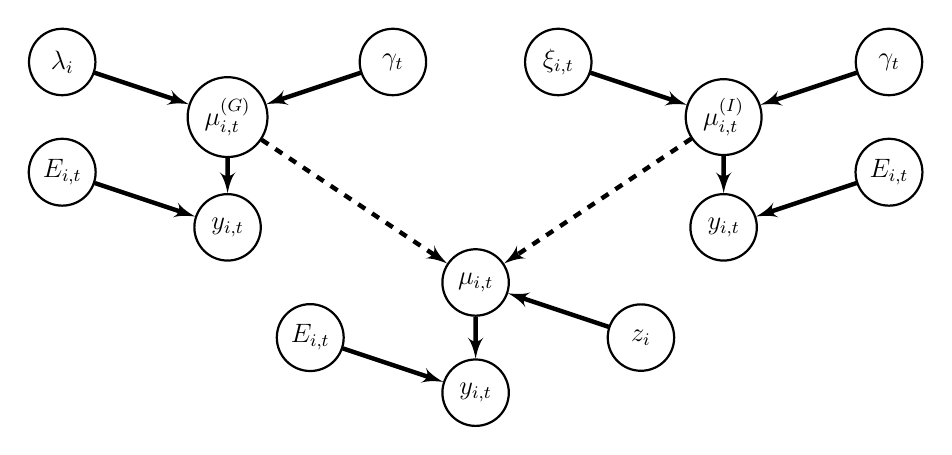
\begin{tikzpicture}[thick,scale=0.7, every node/.style={scale=0.8}]
\tikzset{vertex/.style = {shape=circle,draw,minimum size=3em, thick}}
\tikzset{edge/.style = {ultra thick, ->,> = latex'}}
% main
\node[vertex] (mu) at (9.5,2) {\large$\mu_{i,t}$};
\node[vertex] (y) at  (9.5,0) {\large$y_{i,t}$};
\node[vertex] (E) at  (6.5,1) {\large$E_{i,t}$};
\node[vertex] (z) at  (12.5,1) {\large$z_i$};
% model 1
\node[vertex] (mug) at (5,5) {\large$\mu_{i,t}^{(G)}$};
\node[vertex] (yg) at  (5,3) {\large$y_{i,t}$};
\node[vertex] (Eg) at  (2,4) {\large$E_{i,t}$};
\node[vertex] (gamma) at (8,6) {\large$\gamma_t$};
\node[vertex] (lambda) at (2,6) {\large$\lambda_i$};
% model 2
\node[vertex] (mus) at (14,5) {\large$\mu_{i,t}^{(I)}$};
\node[vertex] (ys) at  (14,3) {\large$y_{i,t}$};
\node[vertex] (Es) at  (17,4) {\large$E_{i,t}$};
\node[vertex] (u) at (17,6) {\large$\gamma_t$};
\node[vertex] (xi) at (11,6) {\large$\xi_{i,t}$};
%edges
\draw[edge] (E) to (y);
\draw[edge] (mu) to (y);
\draw[edge] (z) to (mu);
%edges 1
\draw[edge] (Eg) to (yg);
\draw[edge] (mug) to (yg);
\draw[edge] (gamma) to (mug);
\draw[edge] (lambda) to (mug);
\draw[edge, dashed] (mug) to (mu);
%edges 2
\draw[edge] (Es) to (ys);
\draw[edge] (mus) to (ys);
\draw[edge] (u) to (mus);
\draw[edge] (xi) to (mus);
\draw[edge, dashed] (mus) to (mu);

\end{tikzpicture}
\label{fig:baystdetect}
\caption{Directed acyclic graph showing conditional dependencies between model variables for the BaySTDetect model. Dashed lines indicte one way flow of information. Based on figure in \citet{baystdetect}.}
\end{figure}


\section{Combining the models}

The original computational specification of BaySTDetect was in \emph{BUGS}, using the cut function\footnote{The original BUGS code can be difficult to find on the Journal website: a copy can be found on my Github under /model/bugs/}. The cut function, essentially, makes a copy of the model structure and data \emph{downstream} from the variable and uses standard Gibbs to produce samples of the variable, isolated from the rest of the model. The samples of this variable are then used downstream in the model as specified but are treated as though they came from some fixed distribution. \\

However, this implementation can be improved upon in a number of ways. Firstly, as found by \citep{plummer2015cuts}, the method that is applied in the BUGS software will not converge to a well defined limiting distribution, although there may exist modifications to the algorithm that resolve this. Secondly, as described in section 2545, Gibbs sampling will be very slow to converge to true result -- where Hamiltonian Monte-Carlo may improve on this. And thirdly, the base level of the model is simply a mixture on the rate component of a Poisson random variable -- this can be simplified to a direct calculation by hand. \\

In our implementation we first fit the two models individually in Stan, the code can for this be found in codeblahref. Four chains, with dispersed starting positions, were run for x iterations each for model 1 and y iterations for model 2. Where these numbers was chosen to be a short chain length where the $\hat{R}$ values (the Gelman-Rubin statistic) were consistently $<1.01$ over multiple runs, indicating good convergence. Additionally a visual inspection of the trace plots for some select parameters did not indicate any worrying pathalogical behaviour. \\

We then extracted a sample (without replacement) of the $\mu^{(G)}$ and $\mu^{(I)}$ from the chains and used these to contruct two models
\begin{equation}
P(y_{i,1:T} | M_1, \mu^{(G)}) = \prod_{t=1}^T \frac{{\left(\mu_{i,t}^{(G)}\right)}^{y_{i,t}} \cdot \exp{\left\{-\mu_{i,t}^{(G)}}\right\}}{y_{i, t}!} 
\end{equation}
\begin{equation}
P(y_{i,1:T} | M_2, \mu^{(I)}) = \prod_{t=1}^T \frac{{\left(\mu_{i,t}^{(I)}\right)}^{y_{i,t}} \cdot \exp{\left\{-\mu_{i,t}^{(I)}}\right\}}{y_{i, t}!}.
\end{equation}
That is, the likelihood of the data at each region under each model is that of a series of independent Poisson variables where the rate parameters are decided by one of the samples from either the general or independent trend model. \\

We calculate both these likelihoods, for each region, for every sample of the $\mu$. Then, using these likelihoods we can perform Bayesian model comparison as
\begin{equation}
P(M_j | y_{i, 1:T}) = \frac{P(y_{i, 1:T} | M_2) P(M_2)}{P(y_{i, 1:T})}
\end{equation}
where our prior for the probability of each model being correct follows from the definition of $z_i$ as
\begin{equation}
\begin{array}{cc}
P(M_1) = 0.95 & P(M_2) = 0.05
\end{array}
\end{equation}

We can then, ignoring the denominator as it is the same for both models, compute the unnormalised posteriors for the two models. Comparing these two values, we can assign an indicator to the $z_i$
\begin{equation}
z_i = \left\{%
\begin{array}{ll}
1, & \text{if } 0.95 \cdot P(y_{i,1:T} | M_1) > 0.05 \cdot P(y_{i,1:T} | M_2) \\
0, & \text{otherwise}
\end{array}\right.
\end{equation}

So, $z_i$ is $1$ if the posterior probability of the general model is greater than that of the specific trend model. Finally, we an average of the $z_i$ over the samples and call this $\bar{z}_i$. \\

To test if this procedure works as expected, we take the samples from our \emph{Stan} chains and use them in a BUGS model with the true Bernoulli indicator. Taking the MCMC based posterior mean of the $z_i$ in this gave very similar values to our method. 



\section{Classification and accuracy}

We can use the $\bar{z}_i$ values to classify regions as either `normal' and `unusual'. We could simply say, any regions which are more likely to be `unusual' are classed as such. However given we are performing this for 210 regions we run into issues of multiple comparison. Therefore, \citet{baystdetect} uses the Benjamini-Hochberg procedure to find at which level probability we should classify all with lower probabilities as being `unusual'. This procedure ensures, under some assumptions, that we keep the false discovery rate (FDR) under a given value. \\

With the values we found, explicitly implementing this procedure was not neccesary as a set of 16 regions had $z_i$ values of 0 while the others had much higher values. Of these 16 regions, 15 were the correctly identified unsual regions. Giving a power of 100\% and an FDR of about 0.51\%.

As a sanity check, we look at the samples of $\gamma_t$ from model 1 to see if it approximates the true general temporal trend. A violin plot of the samples can be seen in fig \ref{fig:temporaltrend}. Comparing this trend to that in fig \ref{fig:timeeffects}
\begin{figure}
\centering
\label{fig:temporaltrend}
\includegraphics[width=\textwidth]{global_temporal}
\caption{Violin plot of the samples from $\gamma_t$ in model 1 of BayeSTDetect.}
\end{figure}

\section{Fully Bayesian model}

The BaySTDetect method, as originally applied is clearly very accurate in its identification of the `unusual' regions. Though, the use of the cut function is puzzling. The model, when specified as a true mixture model, essentially describes how the data was generated originally. To test this, we combined the two models as specified without the cut function and fit the entire model in \emph{Stan}. This was done by specifying the probability of the Bernoulli as the Beta prior with mean 0.90 -- allowing the use of HMC and gaining computational efficiency as described in the computational considerations section. \\

The resulting values of $q_i$, however, was barely more accurate than random in ordering the probabilities of each region being `unusual'. In fact, looking at the posterior mean of some the individual temporal trends we found they did not resemble the regions true trend -- even for the `unusual' regions. The following section discusses why this is the case.

\section{The cut function}

The BUGS book describes how the cut function should be used when we wish to prevent the feedback from some response data to the variables that it depends on. For example, in PKPD modelling we have two models which have some shared parameters that are fit to two seperate sets data. It is suggested in \citet{lunn} that the conflict between these two data sources will impede the correct fitting of these parameters if we believe that the two sets of data are quantifying the same underlying feature but one is considered to be a less noisy measurment than the other. In this case, we may wish to prevent the feedback of information from the less accurate data to model based on the more accurate data. At least heuristicaly this might make sense as we dont want the non-shared model parameters of the more accurate model to be affected by the low quality data of the other. Although, as mentioned previously, others may disagree with is model formulation. To quote Andrew Gelman,
\begin{displayquote}
The reason why I (and others) perceive "cut" as bad news is because when you do "cut",  you are no longer doing Bayesian inference.  To put it another way, if it's really true that you don't want inference going from A to B, I don't think you want it going from B to A either.  Joint distributions go both ways.     
\end{displayquote}
It might be more fruitfull to design a prior structure which takes into account the quality of the data, rather than resorting to the breaking of inference. \\

However, to our understanding, this data conflict issue is not present in the BaySTDetect model -- so why do we use the cut function? The original paper \citep{baystdetect} justified its use by asserting it prevents ``double counting'' although it is not clear what this would mean in this context. \\

Evidently the cut model, in some sense, recovers the ground truth better than the fully Bayesian model which seems to describe the data generatively so something must be going on here. We suspect, observing the individual trends, that the trend of each region is being fit primarily via the general trend, with the temporal trends varying wildly in order to influence the posterior density of the regions temporal structure. This leads us to conclude that the fully Bayesian model is not identifiable. This should not come as a surprise. Mixture models are beginning to become notorious for their both idenitfiability issues and difficulty of computation. To quote Michael Betancourt,
\begin{displayquote}
Friends don't let friends fit mixture models, at least not for problems that matter.
\end{displayquote}

When such identifiability arise we can sometimes specify the prior in such a way as to negate the problem. Such as enforcing an ordering to counter the label swithcing problem. In this context though, we are unaware of any prior or restraint which would solve our issue. This could be a useful avenue for future research.

\chapter{Excess variability model}

The second Bayesian model we will look at also attempts to classify the regions, into typical and atypical sets, using a mixture model. I this model, the pathology that defines an atypical areas is not an individual temporal trend, but possesing excessive inseperable spatiotemporal variance. \\

In this paradigm, we use seperate temporal and spatial random effects to capture most ot the heterogeneity between counts. Then any significant space-time interactions that are not common to the shared random effects would indicate a departure from what we would consider typical behaviour. \\

This model primarily based is on the one proposed in \citet{stability}, with two modifications. First, our latent variable works at the regional level -- as opposed to classifying regions based on a decision rule for a mixture component for each count (i.e. we use $z_{i}$ rather than their $z_{i,t}$). And secondly, we take the response as Poisson distributed rather than Binomial as we do not know the population sizes explicitly.

\section{Model specification}

Like in the previous model we model the counts as a Poisson process, $Y_{i,t} \sim \operatorname{Poisson}(E_{i,t} \cdot \mu_{i,t})$, with a rate parameter defined additively on the log-scale
\begin{equation}
\log(\mu_{i,t}) = \lambda_i + \gamma_t + \psi_{i,t}.
\end{equation}

where, as before, the spatial effects are given a BYM prior
\begin{align*}
v_{1:N} &\sim \operatorname{CAR}(W, \sigma_v^2) \\
\lambda_{1:N} &\sim \mathcal{N}(v, I_N \cdot \sigma_\lambda^2) \\
\end{align*}

and the 
\begin{equation*}
\gamma_{1:T} \sim \operatorname{RW}_1(\sigma_\gamma^2).
\end{equation*}

With the new component $\psi$ we wish to capture any residual space-time inseperable heterogeneity in the counts. However, we would expect that the is \emph{some} level of interaction at each region, so we define $\psi$ as the mixture of two normal distributions, with the mixture component at the regional level
\begin{equation}
\psi_{i,t} \sim z_i \cdot \operatorname{Normal}(0, \tau_1^2) + (1 - z_i) \cdot \operatorname{Normal}(0, \tau_2^2)
\end{equation} 
where the first normal mixture captures only minor interactions, to which we do not assign any epidemiological significance, and the second mixture captures that we would consider atypical. \\

The mixture components are each assigned Bernoulli priors 
\begin{equation}
  z_i \sim \operatorname{Bernoulli}(q_i)
\end{equation}

and the $q_i$ are given Uniform priors on (0, 1). Here we are marginilizing out the $z_i$ and instead performing inference on the $q_i$ which confers the advantages set out under the computational considerations section. The variance parameters are given half-normal priors, one a vague prior (representing the abnormal regions) and the other an informative prior which restricts the inseperable variance of the `normal' regions to be very limited. Identification issues and the label switching problem are avoided by defining the larger of the variances addivitely in terms of the smaller:
\begin{align}
  \tau_1 &\sim \operatorname{Normal}(0, 0.01) \cdot I(0, \infty) \\
  k &\sim \operatorname{Normal}(0, 100) \cdot I(0, \infty)
\end{align}
\begin{equation}
 \tau_2 = \tau_2 + k
\end{equation}
where $I$ is the indicator function. \\

The structure of this model, based on the conditional dependencies between variables can be seen in the Bayesian network in fig \ref{fig:bay}. 

Unlike the BaySTDetect model, when we classify the regions in the two sets, we can not use the numerical values of the posterior means of the $q_i$ to define a decision rule by region. This is because the $q_i$ are given uniform priors on the unit interval which does not adequetly convey our prior beliefs that the typical regions should far outnumer the atypical ones. Such a prior could be constructed but a simple Beta prior or similar will not accurately represent this belief. \\

Instead, we select a preselected number of regions ordinally based on these posterior means of the $q_i$.

\section{Classification and accuracy}

This model was fit entirely within \emph{Stan}, as before, and the fifteen regions with the greatest values of $q_i$ were selected as the atypical regions. This procedure correctly identified 11 of the fifteen `unusual' regions giving a false negative rate of 26.7\% and a false positive rate of 2.05\%. This improves on the false positive rate of the CUSUM model but demonstrates much lower power than either CUSUM or BaySTDetect. The performace the method can be seen graphically in fig 1984. \\

Despite the reasonable performance of the \citet{stability} model, it has a number of stark disadvantages compared to BaySTDetect. Firstly, as noted in \citet{baystdetect}
\begin{displayquote}
``However, by construction, this model may not be particularly sensitive when the departures exhibit particular time patterns, for example, higher risks occurring at some consecutive time points.''.
\end{displayquote}

And secondly, the BYM prior has a tendancy to oversmooth the pointwise data -- leading some to develop semiparametric models to counteract this \citep{best2005comparison}.

\begin{figure}
\centering
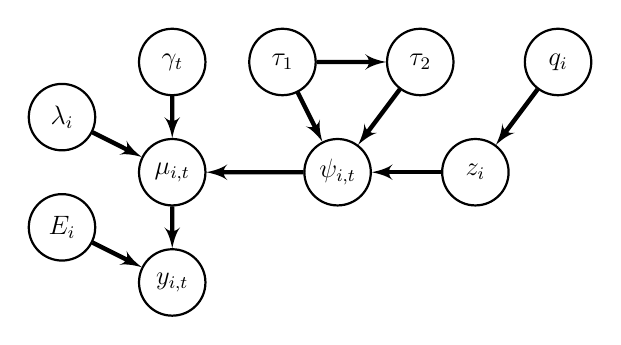
\begin{tikzpicture}[thick,scale=0.7, every node/.style={scale=0.8}]
\tikzset{vertex/.style = {shape=circle,draw,minimum size=3em, thick}}
\tikzset{edge/.style = {ultra thick, ->,> = latex'}}
% main
\node[vertex] (mu) at (8,2) {\large$\mu_{i,t}$};
\node[vertex] (y) at  (8,0) {\large$y_{i,t}$};
\node[vertex] (E) at  (6,1) {\large$E_{i}$};
\node[vertex] (lambda) at  (6,3) {\large$\lambda_i$};

\node[vertex] (gamma) at  (8,4) {\large$\gamma_{t}$};
\node[vertex] (psi) at  (11,2) {\large$\psi_{i,t}$};
\node[vertex] (z) at  (13.5,2) {\large$z_i$};
\node[vertex] (q) at  (15,4) {\large$q_i$};

\node[vertex] (tau1) at  (10,4) {\large$\tau_1$};
\node[vertex] (tau2) at  (12.5,4) {\large$\tau_2$};

%edges
\draw[edge] (mu) to (y);
\draw[edge] (E) to (y);
\draw[edge] (gamma) to (mu);
\draw[edge] (lambda) to (mu);
\draw[edge] (psi) to (mu);
\draw[edge] (z) to (psi);
\draw[edge] (q) to (z);
\draw[edge] (tau1) to (psi);
\draw[edge] (tau2) to (psi);
\draw[edge] (tau1) to (tau2);

\end{tikzpicture}
\label{fig:baystdetect}
\caption{Directed acyclic graph showing conditional dependencies between model variables for the excess variability model. Dashed lines indicte one way flow of information.}
\end{figure}

\begin{figure}
\centering
\includegraphics[width=5in]{variden}
\label{fig:variden}
\caption{Map of unusual regions for the excess variance model. Correctly identified regions are {\color{Green} \bf green}, false-negatives are {\color{Blue}\bf blue} and false-positives are {\color{Red}\bf red}}
\end{figure}

\section{Over-smoothing}

As noted in the previous section, the BYM prior has a tendancy to oversmooth the counts at each regions. This can be of particular hinderance to models such as \citet{spatial}, and the modified version above, as we specifically looking for regions which can not be explained by the spatial smoothing term. This leaves regions that would otherwise have been correctly identified as atypical, deemed typical due to the smooth progression of the spatial heterogeneity locally. \\

Of course, from an epidemiological perspective, the transmission of disease and the dispersed nature of some enviromental hazards would lead us to \emph{expect} pathalogical regions to cluster. Ideally, we need our model that is able to smooth the counts while retaining the ability to identify clustered unusual areas.

\section{Simulated Data}

We test the severity of this issue of generating a new set of simulated data where the unusual areas are clustered together. \\

In order to generate the list of unusual areas we suggest a simple algorithm inspired by preferential attatchment processes in network theory. The method is as follows
\begin{enumerate}
\item Construct a list of the regions and a corresponding list of `weights'. 
\item Assign all regions $i$ an initial weight of $1$ and set $k=1$.
\item Select a new region $u_k$ from the list of potential regions with probability corresponding to the categorical distribution defined by
\begin{equation}
P(u_k = j) = \frac{w_j}{\sum_{i} w_i}
\end{equation}
\item Mark the selected region as unusual and remove it (and its weight) from the list of potential regions.
\item Add $w^*$ to each region $i$ that was adjacent to the region removed
\begin{equation}
w_i = w_i + w^* \ \ \forall i \in \partial u_k
\end{equation}
where we call $w^*$ the preference weight.
\item Increment $k$ and return to step 3 until the desired number of unusual regions have been selected. 
\end{enumerate}

This procedure was applied to the shape data of the 210 CCGs with a preference weight of $w^* = 20$ to select 15 regions in total. The resulting unusual regions selected can be seen in fig \ref{fig:unusual}. We see that the selected regions form a series of clusters of varying sizes. \\

Using this list of unusual regions we proceeded to generate the data as follows. A random walk was simulated
\begin{equation*}
\gamma_{1:15} \sim \operatorname{RW}_1(0.1^2)
\end{equation*}
and then normalised to have a mean of zero. The deviant temporal trend was created generated by adding seperate half-normal variables to the final six time points of the general trend. The resulting two trends can be seen in fig \ref{fig:unusual}. \\

The spatial component was simulated from a BYM prior and was combined with the temporal trend, identically to as in Chapter 2, to create the rate variables for each region and time point. Multiplying by the same expected values as previously, we drew from a Poisson distribution to arrive at the final values. The code for this can be found in the appendix. \\

Now applying the same procedure as described earlier in the chapter, we only 3 of the total 15 regions were correctly identified. For a null hypothesis where we select the atypical regions randomly, this number of identified regions would give a p-value of around 8\%\footnote{\> 1 - phyper(2, 15, 195, 15) = 0.07968} -- not very good! Examining the regions identified in fig 321, we that the regions we did correctly identify are non-contiguous. Futher confirming our hypothesis that this method will fail to identify unusual areas when they cluster together.


\begin{figure}
\centering
\includegraphics[width=5in]{preftemporal}
\label{fig:preftemporal}
\caption{Simulated temporal trend for data with clustered unusual regions. The general temporal trend is blue and the red line shows the departure that the deviant trend exhibits.}
\end{figure}

\begin{figure}
\centering
\subfloat[Truly unsual regions]{\includegraphics[width=0.5\textwidth]{trueunusual}}
\subfloat[Model classification]{\includegraphics[width=0.5\textwidth]{var}}
\label{fig:unusual}
\caption{Map of unusual regions for the excess variance model where there are clustered unusual regions. Correctly identified regions are {\color{Green} \bf green}, false-negatives are {\color{Blue}\bf blue} and false-positives are {\color{Red}\bf red}}
\end{figure}

\chapter{Computational considerations}

In this chapter we briefly note some of the computational considerations that one should be cogent of for some the methods used in this project.

\section{Computational software}

Pymc3 was first used to fit the Bayesian models as it has the advantage of both using HMC for continuous variables and other sampling routines, e.g. slice, for discrete variables. However, we ran into intractable computational issues. A discussion of this with the developers can be found here: https://github.com/pymc-devs/pymc3/issues/1652. \\

Instead Stan was used throughout the project to fit continuous variables. As an aside, we attempted to use auto-diff variational inference but the uncorrelated form did not fit well and the full rank model was too slow to fit.
 

\section{Reparameterization of the models}

Removing conditional dependencies can be used to reduce local dependence between variables -- improving the exploration of the sample space.

\begin{align*}
\lambda \sim N(v, \sigma^2_\lambda) = N(0, 1) \cdot \sigma_\lambda^2 + v
\end{align*}


\section{Marginilizing over the discrte parameters}

As \emph{Stan} uses Hamiltonian Monte-Carlo, which is a gradient based sampler, we can't directly specify a discrete prior as used in mixture models. Instead we can ``marginalize out'' the mixture component to obtain a purely continuous distribution. This also confers some computational benefits in terms of the speed at which the chain converges due to the Rao-Blackwellization of the estimator \citep{rao}. \\

Take for example a mixture of two Normal distributions
\begin{equation}
  k \cdot \operatorname{Normal(\mu_1, \sigma_1^2)} + (1 - k) \cdot \operatorname{Normal(\mu_2, \sigma_2^2)}
\end{equation} 
\begin{equation}
  k \sim \operatorname{Bernoulli(\lambda)}.
\end{equation}

In Monte-Carlo we simply need to be able to calculate the posterior at a specific point. Most software, including \emph{Stan}, rather than multiply the posterior by a chain of conditional probability density functions works on the $\log$ scale where to calculate the log posterior we simply need to increment the log posterioir by the log conditional of the hierachical components. So for our mixture of Normals we need to implement the following
\begin{align}
  \text{log\_posterior} &= \text{log\_posterior} + \log(\lambda \cdot \operatorname{Normal\_pdf}(x | \mu_1, \sigma_1^2)  \nonumber \\
                   & \ \ + (1 - \lambda) \cdot \operatorname{Normal\_pdf}(x | \mu_2, \sigma_2^2))
\end{align}

which we can see is continuous. The way we can specifically implement this in \emph{Stan} is by using the following manipulation

\begin{align}
\log(p_X(x | \lambda, \mu_i, \sigma^2_i)) &= \log(\lambda \cdot \operatorname{Normal\_pdf}(x | \mu_1, \sigma_1^2)  \nonumber \\
& \ \ \ \ \ \ \ + (1 - \lambda) \cdot \text{Normal\_pdf}(x | \mu_2, \sigma_2^2)) \\
&= \log(\exp(\log(\lambda \cdot \operatorname{Normal\_pdf}(x | \mu_1, \sigma_1^2)))  \nonumber \\
& \ \ \ \ \ \ \ + \exp(\log((1 - \lambda) \cdot \operatorname{Normal\_pdf}(x | \mu_2, \sigma_2^2)))) \\
&= \operatorname{log\_sum\_exp}(\log(\lambda) + \log\operatorname{Normal\_pdf}(x | \mu_1, \sigma_1^2),  \nonumber \\
& \ \ \ \ \ \ \ \log(1 - \lambda) + \log\operatorname{Normal\_pdf}(x | \mu_2, \sigma_2^2))
\end{align} 

For more on this see page 185 of \cite{stan}.

\chapter{Comparisions and conclusions}

We now consider the relative benefits of each of the techniques we have implemented and suggest some natural avenues by which the models could be improved. A summary of the timing, false-postive and false-negative rates can be found in table \ref{fig:table}. \\

The CUSUM procedure, as we have defined, shows excellent sensitivity to the types of pathologies that we which to detect. However, the model performes relatively poorly in terms of specificity -- with the highest false-positive rate of the three techniques. The use of an adaptation to the model, such as the spatial CUSUM, could further improve the model in this respect by the shrinkage granted by a smoothing procedure. \\

Furthermore, the speed at which the CUSUM--as implemented--performs the classification may suit it better to applications where the length of the time interval or the number of regions render the analogous Bayesian methods impractical. \\

The excess variance model performs reasonably well in terms of sensitivity and specificity, although it is outclassed in both of these respects compared to the BaySTDetect model. Though this is to be expected as the generation of the data followed a very similar form to the latter. While we are testing the abilities of the models to detect an unusal temporal trend it is unclear whether such a pathology is truly indicative of those which are epidemiologically significant. Additionaly, the fully Bayesian nature of the variance model may make the interpretation of both the model parameters and the addition of any futher complexity more straightforward. \\

However, we have shown that this model will fall short when we wish to detect a group of unusual areas which are tightly clustered together due to the oversmoothing caused by the BYM prior. Perhaps, as suggested in \cite{best2005comparison}, the model could be improved by the use of a semi-parametric specification of the spatial component or, as mentioned in \cite{bym}, the use of a prior with a different distance metric as both would allow for discontinuities in the risk surface. \\

The BaySTDetect model clearly performs the best on this data but the neccesity of the cut function should be explored further to see if there is a prior structure which allows for a greater independence between the fitting of the geenral and specific temporal trends. Moreover, the fitting of an individual trend to each region is extremely compuationally expensive and may become unfeasible as the number of regions grows. \\

With regards to the timing of the methods, a like-for-like comparison with BUGS was not possible as OpenBUGS had to be used through a compatability layer (WINE) due to operating system requirements over certain aspects of the GeoBUGS package. This disclaimer aside, the original implementation of the BaySTDetect algorithm in \citet{baystdetect} was ran in BUGS to a length that generated a similar effective sample size to that used in Stan. The chains took a number of hours generate these samples---an order of magnitude slower than in Stan---and the Gelman-Rubin statistics, while within reasonable bounds, were not as low as in Stan. \\

Therefore, we have shown that the use of Stan in epidemiological models is both feasable and advantageous over typical implementations. Also note that computational time should scale much better under Hamiltonial Monte-Carlo than under Gibbs and Metropolis-Hastings as outlined earlier, suggesting that for larger and more complex models, that may be explored in the future, software such as Stan may be uniquely suited.

\bgroup
\def\arraystretch{1.5}%
\begin{figure}
\centering
\begin{tabular}{| c | c | c | c |}
\hline
Method & False-positive rate (\%) & False-negative rate (\%) & Wall time (seconds) \\ \hline
CUSUM & 5.12 & 0.00 & 34 \\ \hline
BaySTDetect & 0.512 & 0.00 & 1944 \\ \hline
Excess Variance & 2.05 & 26.7 & 720 \\
\hline
\end{tabular}
\label{fig:table}
\caption{Comparison of the methods implemented on the simualted data.}
\end{figure}
\egroup

\chapter{Code appendix}

There is far too much code in this project to fit in the appendix. To code for the entire project can be found on my Github at https://github.com/michaelaredman/Masters-Project. A \textbf{very} select subset of the code is included here

\begin{minted}
functions {
  /**
  * This part is taken from Max Joseph's write-up here: http://mc-stan.org/documentation/case-studies/mbjoseph-CARStan.html
  *
  * Return the log probability of a proper conditional autoregressive (CAR) prior 
  * with a sparse representation for the adjacency matrix
  *
  * @param phi Vector containing the parameters with a CAR prior
  * @param tau Precision parameter for the CAR prior (real)
  * @param alpha Dependence (usually spatial) parameter for the CAR prior (real)
  * @param W_sparse Sparse representation of adjacency matrix (int array)
  * @param n Length of phi (int)
  * @param W_n Number of adjacent pairs (int)
  * @param D_sparse Number of neighbors for each location (vector)
  * @param lambda Eigenvalues of D^{-1/2}*W*D^{-1/2} (vector)
  *
  * @return Log probability density of CAR prior up to additive constant
  */
  real sparse_car_lpdf(vector phi, real tau, real alpha, 
    int[,] W_sparse, vector D_sparse, vector lambda, int n, int W_n) {
      row_vector[n] phit_D; // phi' * D
      row_vector[n] phit_W; // phi' * W
      vector[n] ldet_terms;
    
      phit_D = (phi .* D_sparse)';
      phit_W = rep_row_vector(0, n);
      for (i in 1:W_n) {
        phit_W[W_sparse[i, 1]] = phit_W[W_sparse[i, 1]] + phi[W_sparse[i, 2]];
        phit_W[W_sparse[i, 2]] = phit_W[W_sparse[i, 2]] + phi[W_sparse[i, 1]];
      }
    
      for (i in 1:n) ldet_terms[i] = log1m(alpha * lambda[i]);
      return 0.5 * (n * log(tau)
                    + sum(ldet_terms)
                    - tau * (phit_D * phi - alpha * (phit_W * phi)));
  }
}
data {
    int<lower = 1> numRegions; // The number of regions
    int<lower = 1> nt; // The number of time points
    // matrix[numRegions, nt] observed;  // The observed counts at each point
    int observed[numRegions, nt];
    vector[numRegions] log_expected; // The expected number of counts based on demographics etc
    matrix<lower = 0, upper = 1>[numRegions, numRegions] W; // The adjacency matrix
    int W_n;
}
transformed data{
    int W_sparse[W_n, 2];   // adjacency pairs
    vector[numRegions] D_sparse;     // diagonal of D (number of neigbors for each site)
    vector[numRegions] lambda;       // eigenvalues of invsqrtD * W * invsqrtD
    
    { // generate sparse representation for W
	int counter;
	counter = 1;
	// loop over upper triangular part of W to identify neighbor pairs
	for (i in 1:(numRegions - 1)) {
	    for (j in (i + 1):numRegions) {
		if (W[i, j] == 1) {
		    W_sparse[counter, 1] = i;
		    W_sparse[counter, 2] = j;
		    counter = counter + 1;
		}
	    }
	}
    }
    for (i in 1:numRegions) D_sparse[i] = sum(W[i]);
    {
	vector[numRegions] invsqrtD;  
	for (i in 1:numRegions) {
	    invsqrtD[i] = 1 / sqrt(D_sparse[i]);
	}
	lambda = eigenvalues_sym(quad_form(W, diag_matrix(invsqrtD)));
    }
}
parameters {
    vector[nt] temporal;
    vector[numRegions] v; // Spatial smoothing component
    vector[numRegions] lmbda;
    //real cons;
    real<lower = 0> sigma_v; // Variance of spatial component, v
    real<lower = 0> sigma_temporal; // Variance of temporal component
    real<lower = 0> sigma_l;
    real<lower=0, upper=1> alpha;

}
transformed parameters {

    matrix[numRegions, nt] mu_general;
    
    mu_general = rep_matrix(log_expected, nt) + rep_matrix(lmbda, nt) + rep_matrix(temporal, numRegions)';
    //mu_general = rep_matrix(log_expected, nt) + rep_matrix(lmbda, nt) + rep_matrix(temporal, numRegions)' + rep_matrix(cons, numRegions, nt);
    
}
model {
    sigma_temporal ~ normal(0, 1);
    sigma_v ~ normal(0, 1);
    sigma_l ~ normal(0, 1);
    
    temporal[1] ~ normal(0, sigma_temporal); // 1d random walk prior on temporal component
    for (t in 2:nt) {
	temporal[t] ~ normal(temporal[t - 1], sigma_temporal);
    }
    
    //cons ~ normal(0, 30); // constant term for general
    
    v ~ sparse_car(sigma_v, alpha, W_sparse, D_sparse, lambda, numRegions, W_n);
    lmbda ~ normal(v, sigma_l);
    
    for (t in 1:nt) {
	observed[,t] ~ poisson_log(mu_general[,t]);
    }
    
}
\end{minted}

\begin{minted}{r}
data {
    int<lower = 1> numRegions; // The number of regions
    int<lower = 1> nt; // The number of time points
    int observed[numRegions, nt];
    vector[numRegions] log_expected; // The expected number of counts based on demographics etc
}
parameters {
    real<lower = 0> var_ind_temporal[numRegions]; // The variance of the individual temporal trends
    
    matrix[numRegions, nt] ind_temporal; // The temporal trend of an individual region
    vector[numRegions] ind_constant;

    real a;
    real<lower = 0> b;
}
transformed parameters {
    matrix[numRegions, nt] mu_specific;
    
    mu_specific = ind_temporal + rep_matrix(ind_constant, nt) + rep_matrix(log_expected, nt);
}
model {
    
    ind_temporal[,1] ~ normal(0, sqrt(var_ind_temporal)); 
    for (t in 2:nt) {
	ind_temporal[,t] ~ normal(ind_temporal[, t - 1], sqrt(var_ind_temporal));
    }

    ind_constant ~ normal(0, 30); // non-informative prior on the constant term per region

    var_ind_temporal ~ lognormal(a, b);
    a ~ normal(0, 30);
    b ~ normal(0, 2.5);
    
    for (t in 1:nt) {
	observed[,t] ~ poisson_log(mu_specific[,t]);
    }

}

\end{minted}

\begin{minted}{r}
functions {
  /**
  * This part is taken from Max Joseph's write-up here: http://mc-stan.org/documentation/case-studies/mbjoseph-CARStan.html
  *
  * Return the log probability of a proper conditional autoregressive (CAR) prior 
  * with a sparse representation for the adjacency matrix
  *
  * @param phi Vector containing the parameters with a CAR prior
  * @param tau Precision parameter for the CAR prior (real)
  * @param alpha Dependence (usually spatial) parameter for the CAR prior (real)
  * @param W_sparse Sparse representation of adjacency matrix (int array)
  * @param n Length of phi (int)
  * @param W_n Number of adjacent pairs (int)
  * @param D_sparse Number of neighbors for each location (vector)
  * @param lambda Eigenvalues of D^{-1/2}*W*D^{-1/2} (vector)
  *
  * @return Log probability density of CAR prior up to additive constant
  */
  real sparse_car_lpdf(vector phi, real tau, real alpha, 
    int[,] W_sparse, vector D_sparse, vector lambda, int n, int W_n) {
      row_vector[n] phit_D; // phi' * D
      row_vector[n] phit_W; // phi' * W
      vector[n] ldet_terms;
    
      phit_D = (phi .* D_sparse)';
      phit_W = rep_row_vector(0, n);
      for (i in 1:W_n) {
        phit_W[W_sparse[i, 1]] = phit_W[W_sparse[i, 1]] + phi[W_sparse[i, 2]];
        phit_W[W_sparse[i, 2]] = phit_W[W_sparse[i, 2]] + phi[W_sparse[i, 1]];
      }
    
      for (i in 1:n) ldet_terms[i] = log1m(alpha * lambda[i]);
      return 0.5 * (n * log(tau)
                    + sum(ldet_terms)
                    - tau * (phit_D * phi - alpha * (phit_W * phi)));
  }
}
data {
    int<lower = 1> numRegions; // The number of regions
    int<lower = 1> nt; // The number of time points
    // matrix[numRegions, nt] observed;  // The observed counts at each point
    int observed[numRegions, nt];
    vector[numRegions] log_expected; // The expected number of counts based on demographics etc
    matrix<lower = 0, upper = 1>[numRegions, numRegions] W; // The adjacency matrix
    int W_n;
    real<lower = 0, upper = 1> alpha; //The degree of spatial dependence
}
transformed data{
    int W_sparse[W_n, 2];   // adjacency pairs
    vector[numRegions] D_sparse;     // diagonal of D (number of neigbors for each site)
    vector[numRegions] lambda;       // eigenvalues of invsqrtD * W * invsqrtD
    
    { // generate sparse representation for W
	int counter;
	counter = 1;
	// loop over upper triangular part of W to identify neighbor pairs
	for (i in 1:(numRegions - 1)) {
	    for (j in (i + 1):numRegions) {
		if (W[i, j] == 1) {
		    W_sparse[counter, 1] = i;
		    W_sparse[counter, 2] = j;
		    counter = counter + 1;
		}
	    }
	}
    }
    for (i in 1:numRegions) D_sparse[i] = sum(W[i]);
    {
	vector[numRegions] invsqrtD;  
	for (i in 1:numRegions) {
	    invsqrtD[i] = 1 / sqrt(D_sparse[i]);
	}
	lambda = eigenvalues_sym(quad_form(W, diag_matrix(invsqrtD)));
    }
}
parameters {
    vector[nt] temporal;
    vector[numRegions] v; // Spatial smoothing component
    vector[numRegions] lmbda; 
    real<lower = 0> sigma_v; // Variance of spatial component, v
    real<lower = 0> sigma_temporal; // Variance of temporal component
    real<lower = 0> sigma_l;
    //real constant;
    //real<lower = 0, upper = 1> alpha; // The degree of spatial dependence - implicitly given flat prior

    vector<lower = 0, upper = 1>[numRegions] indicator; // Mixture component
    matrix[numRegions, nt] xi; // Space-time inseperable component

    real<lower = 0> tau_1;
    real<lower = 0> k;
    

}
transformed parameters {
    real<lower = 0> tau_2;
    matrix[numRegions, nt] mu;

    tau_2 = tau_1 + k;

    //mu = rep_matrix(constant, numRegions, nt) + rep_matrix(temporal, numRegions)' + rep_matrix(lmbda, nt) + rep_matrix(log_expected, nt) + xi
    mu = rep_matrix(temporal, numRegions)' + rep_matrix(lmbda, nt) + rep_matrix(log_expected, nt) + xi;

}
model {
    sigma_temporal ~ normal(0, 1);
    sigma_v ~ normal(0, 1);
    sigma_l ~ normal(0, 1);
    
    temporal[1] ~ normal(0, sigma_temporal); // 1d random walk prior on temporal component
    for (t in 2:nt) {
	temporal[t] ~ normal(temporal[t - 1], sigma_temporal);
    }
    
    //constant ~ normal(0, 30);

    v ~ sparse_car(sigma_v, alpha, W_sparse, D_sparse, lambda, numRegions, W_n);
    lmbda ~ normal(v, sigma_l);

    indicator ~ beta(0.3, 0.6);

    tau_1 ~ normal(0, 0.1);
    k ~ normal(0, 10);

    for (i in 1:numRegions){
	target += log_sum_exp(log1m(indicator[i]) + normal_lpdf(xi[i,] | 0, tau_1),
			      log(indicator[i]) + normal_lpdf(xi[i,] | 0, tau_2));
	
    }

    for (i in 1:numRegions){
	observed[i,] ~ poisson(exp(mu[i,]));
    }

}

\end{minted}

\begin{minted}{python}

import pandas as pd
import numpy as np
import math
from cusum import cusum as cs
import logging
from matplotlib import pyplot as plt

def load_data():
    temp_expected = pd.read_csv('../../data/csv/expected.csv')
    E = np.array(temp_expected['x'])
    
    temp_sim = pd.read_csv('../../data/csv/simulated.csv')
    temp_times = temp_sim[['Time1', 'Time2', 'Time3', 'Time4', 'Time5', 'Time6', 'Time7', 'Time8', 'Time9', 'Time10', 'Time11', 'Time12', 'Time13', 'Time14', 'Time15']]
    observed_values = np.array(temp_times, dtype=np.int)
    
    numRegions = observed_values.shape[0] #number of regions
    nt = observed_values.shape[1] #number of time points
    
    return numRegions, nt, E, observed_values

numRegions, nt, E, observed_values = load_data()

logger = logging.getLogger("cusum")
logging.basicConfig(level=logging.DEBUG)

class cusum:

    def __init__(self, observed, expected, seed=None):
        self.observed = np.array(observed)
        self.expected = np.array(expected)

        np.random.seed(seed=seed)

        self.numRegions = self.observed.shape[0]
        self.nt = self.observed.shape[1]

        self._calc_expected_trends()

        #default alpha (ratio of in-control to out-of-control rates)
        self.alpha = 1.5
        #default size (number of times to simulated trend to find h value)
        self.size = 4000
        
    def _norm_by_expectation(self):
        """
        Return the observed values divided by their expected values
        """
        return np.array([obs/self.expected[i] for i, obs in enumerate(self.observed)])

    def _general_trend(self):
        """
        Return the mean temporal trend for a process of unit expectation
        """
        return self._norm_by_expectation().mean(axis=0)

    def _calc_expected_trends(self):
        """
        Calculate the temporally adjusted expectations for each region
        """
        general_trend = self._general_trend()
        self.expected_trend = np.zeros(shape=(self.numRegions, self.nt))
        for i in range(self.numRegions):
            self.expected_trend[i, :] = self.expected[i] * general_trend 

    def control_chart(self, time_series, expectation, alpha):
        """
        Calls Fortran subroutine to return the CUSUM control chart for the a given time series
        which is assumed to be a Poisson distributed with given rate parameters.

        Inputs
        ------
        time_series : array (len_series)
            Time series which generates the control chart
        
        expectation : array (len_series)
            In-control rate parameter at each time step 

        alpha : real > 1
            Ratio of in-control rate to out-of-control rate

        Output
        ------
        control_chart : array (len_series)
            The desired control chart.
        """
        control_chart = cs.control_chart(time_series, expectation, alpha)
        return control_chart

    def simulate_trend(self, expectation, size):
        """
        Simulate a Poisson r.v., for a given temporal expectation, (size) times.
        """
        trends = np.zeros(shape=(size, len(expectation)))
        for i in range(len(expectation)):
            trends[:, i] = np.random.poisson(expectation[i], size=size)
        return trends

    def find_h(self, expectation, size, alpha, h_values, p_value):
        simulated_series = self.simulate_trend(expectation, size)
        false_positive_rates = cs.false_positive(simulated_series, expectation, alpha, h_values)
        try:
            my_h = next(h for h, rate in zip(h_values, false_positive_rates) if rate < p_value)
        except StopIteration:
            logger.warning("Unable to find suitable h value. False positive rates were as follows:")
            logger.warning(np.array2string(false_positive_rates))
            my_h = 0
            
        return my_h
        
    def generate_h(self, h_values, p_value):
        temp = []
        for regional_expectation in self.expected_trend:
            new_value = self.find_h(regional_expectation, self.size, self.alpha, h_values, p_value=p_value)
            temp.append(new_value)
        self.h_array = np.array(temp)

    def test(self):
        flags = np.zeros(shape=self.numRegions)
        for i in range(self.numRegions):
            c_chart = cs.control_chart(self.observed[i, :], self.expected_trend[i, :], alpha=self.alpha)
            flags[i] = cs.flag(c_chart, self.h_array[i])
        return flags

    def test_regions(self):
        flags = self.test()
        return np.where(flags == 1)[0]
        


csum = cusum(observed_values, E)
csum.generate_h(np.linspace(0, 10, 250), p_value=0.01)
unusual_predicted = csum.test_regions() + 1

\end{minted}

\begin{minted}{fortran}
module cusum

contains

    function log_likelihood(x, lmbda)
        !! Poisson log-likelihood up to a constant
        implicit none
        real(kind=8), intent(in) :: x, lmbda
        real(kind=8) :: log_likelihood

        log_likelihood = -lmbda + x*log(lmbda)
        
    end function log_likelihood

    function log_likelihood_ratio(x, in_control, out_control)
      !! Difference between the log-likelihoods of the in-control and out-of-control rate models  
      implicit none
      real(kind=8), intent(in) :: x, in_control, out_control
      real(kind=8) :: numerator, denominator, log_likelihood_ratio
      numerator = log_likelihood(x, out_control)
      denominator = log_likelihood(x, in_control)

      log_likelihood_ratio = numerator - denominator
      
    end function log_likelihood_ratio

    subroutine control_chart(time_series, expectation, alpha, S)
      implicit none
      real(kind=8), intent(in) :: alpha
      real(kind=8), dimension(:), intent(in) :: time_series, expectation
      !f2py depend(time_series) S
      real(kind=8), intent(out), dimension(size(time_series)) :: S
      integer :: i, series_len

      series_len = size(time_series)

      S(1) = log_likelihood_ratio(time_series(1), expectation(1), expectation(1)*alpha)
      do i=2,series_len
         S(i) = max(0d0, log_likelihood_ratio(time_series(i), expectation(i), expectation(i)*alpha))
      end do
      
    end subroutine control_chart

    function flag(chart, h)
      implicit none
      real(kind=8), intent(in), dimension(:) :: chart
      real(kind=8), intent(in) :: h
      logical :: flag

      flag = maxval(chart) > h

    end function flag

    subroutine false_positive(simulated_series, expectation, alpha, h_values, fp_rate)
      implicit none
      real(kind=8), intent(in) :: alpha
      real(kind=8), intent(in), dimension(:) :: expectation, h_values
      real(kind=8), intent(in), dimension(:, :) :: simulated_series
      !f2py depend(h_values) fp_rate
      real(kind=8), intent(out), dimension(size(h_values)) :: fp_rate
      integer :: i, j, h_values_len, series_len, num_series
      real(kind=8) :: h
      real(kind=8), dimension(:), allocatable :: chart, ones_list, zeros_list
      logical, dimension(:), allocatable :: flag_list

      h_values_len = size(h_values)
      series_len = size(simulated_series, 2)
      num_series = size(simulated_series, 1)

      allocate(flag_list(num_series))
      allocate(chart(series_len))

      allocate(ones_list(num_series))
      allocate(zeros_list(num_series))
      ones_list = 1.0d0
      zeros_list = 0.0d0

      do i=1,h_values_len
         h = h_values(i)
         do j=1,num_series
            call control_chart(simulated_series(j, :), expectation, alpha, chart)
            flag_list(j) = flag(chart, h)
         end do
         fp_rate(i) = sum(merge(ones_list, zeros_list, flag_list))/num_series
      end do

    end subroutine false_positive
    
end module cusum
\end{minted}

\begin{minted}{python}
import pystan
import pandas as pd
import numpy as np
import time
import pickle
import seaborn as sns
from matplotlib import pyplot as plt

def load_data():
    temp_expected = pd.read_csv('../../data/csv/expected.csv')
    E = np.array(temp_expected['x'])
    
    temp_sim = pd.read_csv('../../data/csv/simulated.csv')
    temp_times = temp_sim[['Time1', 'Time2', 'Time3', 'Time4', 'Time5', 'Time6', 'Time7', 'Time8', 'Time9', 'Time10', 'Time11', 'Time12', 'Time13', 'Time14', 'Time15']]
    observed_values = np.matrix(temp_times, dtype=np.int)
    
    adj = pd.read_csv('../../data/csv/adjacency.csv', index_col=0)
    W = np.matrix(adj)
    
    numRegions = observed_values.shape[0] #number of regions
    nt = observed_values.shape[1] #number of time points
    
    alpha = 0.9 #this was 1 in the model but that makes the covariance matrix singular

    return numRegions, nt, E, W, alpha, observed_values

numRegions, nt, E, W, alpha, observed_values = load_data()

model_data = {'numRegions': numRegions,
              'nt': nt,
              'observed': observed_values,
              'log_expected': np.log(E),
              'W_n': int(W.sum()/2.0),
              'W': W,
              'alpha': alpha}

print('Starting fit at: ', time.ctime())

iter_num = 2000

fit = pystan.stan(file='var.stan', data=model_data, iter=iter_num, chains=4)

print('Finished fit at: ', time.ctime())

trace = fit.extract()

ts = time.localtime()
file_name = "trace/model_{}-{}-{}__{}-{}.pkl".format(ts[2], ts[1], ts[0], ts[3], ts[4])

with open('summary.txt', 'w') as f:
    print(fit, file=f)

with open(file_name, 'wb') as f:
    pickle.dump(trace, f)

true_unusual = pd.read_csv('../../data/csv/unusual.csv')
unusual_regions = np.array(true_unusual['x'])

indicator = trace['indicator']
indicator_av = pd.DataFrame(indicator.mean(axis=0))

indicator_av.index = range(1, 211)
predictor = indicator_av.sort(0)
regions = np.array(predictor.index)

np.savetxt('predicted.csv', regions, delimiter=',', fmt='%i')

fifteen = regions[-15:]

regions_identified = set(unusual_regions).intersection(fifteen)

num_regions_identified = len(regions_identified)
\end{minted}

\begin{minted}{r}
library(maptools)
library(CARBayesdata)
library(rgdal)
library(spdep)
library(MASS)
library(classInt)
library(RColorBrewer)
setwd("~/4th Year/project/data/shapefiles")
shape.basic <- readOGR('.', 'CCG_BSC Feb2013  (clipcoast 200m)')
shape_deathtowales <- shape.basic[shape.basic@data$CCGname != 'Wales',]
shape <- shape_deathtowales[shape_deathtowales@data$CCGname != 'NHS Isle of Wight CCG',]
load("~/4th Year/project/data/rdata/expected_data.Rda")
asthma <- asthma_expected_i[asthma_expected_i$CCG != '10L',]
expected = as.vector(asthma['E']$E)

unusual_temp <- read.csv('~/4th Year/project/data/csv/prefUnusual.csv', header=FALSE)
unusual <- sort(unusual_temp$V1) + 1 #add one as python had zero index

numRegions <- length(shape@data$SP_ID)
cols <- rep('white', numRegions)
cols[unusual] <- rep('yellow', length(unusual))

plot(shape, col=cols)

random_walk <- function(len, sigma) {
  walk <- rep(0, len)
  walk[1] <- rnorm(1, sd=sigma)
  for(i in 2:len) {
    walk[i] <- walk[i-1] + rnorm(1, sd=sigma)
  }
  return(walk)
}

set.seed(314)

rwalk <- random_walk(len=15, sigma=0.1)
rwalk <- rwalk - mean(rwalk)

rwalk_unusual <- rwalk
rwalk_unusual[10:15] <- rwalk_unusual[10:15] + abs(rnorm(n=6, sd = 0.3))

plot(rwalk_unusual, type='l', col='red', ylab = 'Temporal trend', xlab = 't')
lines(rwalk, type='l', col='blue')

neib <- poly2nb(shape)
adj <- nb2mat(neib, style="B") 
num.neib <- colSums(adj)
alpha <- 0.9
prec.matrix <- diag(num.neib) - alpha*adj
cov.matrix <- solve(prec.matrix)
spatial.sd <- 0.02

CAR <- mvrnorm(mu=rep(0, length(num.neib)), Sigma=cov.matrix*spatial.sd)

class <- classIntervals(CAR, 9, style="quantile")
display.brewer.pal(name = "YlOrRd", n=9)
plotclr <- brewer.pal(9,"YlOrRd")
colcode <- findColours(class, plotclr)
plot(shape, col=colcode)

mu <- matrix(data=0, nrow=210, ncol=15)
for(i in 1:210) {
  mu[i, ] <- mu[i, ] + rwalk
}
for(i in unusual) {
  mu[i, ] <- rwalk_unusual
}
for(i in 1:15) {
  mu[, i] <- mu[, i] + CAR + log(expected)
}
rate.matrix <- exp(mu)

pois <- function(lambda) {rpois(n=1, lambda)}
simulated <- apply(rate.matrix, MARGIN=c(1, 2), FUN=pois)
write.csv(simulated, '~/4th Year/project/data/csv/simulated_spatial_corr.csv')

for(i in 1:15) {
  class2 <- classIntervals(simulated[,i], 9, style="quantile")
  plotclr2 <- brewer.pal(9,"YlOrRd")
  colcode2 <- findColours(class2, plotclr2)
  plot(shape, col=colcode2)
}




\end{minted}


\begin{minted}{python}
import numpy as np
import pandas as pd

np.random.seed(21)

adj = pd.read_csv('../data/csv/adjacency.csv', index_col=0)
W = np.matrix(adj)

class generate_unusual:
    """
    Iterative selector for regions from an adjacency matrix with preferential attatchment
    """
    
    def __init__(self, adj, pref_weight=1):

        self.adj = adj
        self.num_regions = adj.shape[0]
        self.pref_weight = pref_weight

        self.nodes = np.array(range(self.num_regions))
        self.weights = np.ones(self.num_regions)
        self.unusual = []

        self.form_probabilities()

    def form_probabilities(self):
        """
        Calculate the vector of probabilities corresponding to each region being picked as the next regions to be selected
        """
        total_weight = self.weights.sum()
        self.prob = np.array([weight/total_weight for weight in self.weights])

    def select_node(self):
        new_node = np.random.choice(self.nodes, p = self.prob)
        return new_node

    def remove_node(self, new_node):
        index = np.where(self.nodes == new_node)[0][0]
        self.nodes = np.delete(self.nodes, index)
        self.weights = np.delete(self.weights, index)

    def update_weights(self, new_node):
        new_node_adj = np.array(self.adj[new_node])[0]
        neib = np.where(new_node_adj == 1)[0]
        #get the indicies of each neighbour in the remaining list of nodes
        indicies = np.concatenate([np.where(self.nodes == node)[0] for node in neib]) 
        self.weights[indicies] = self.weights[indicies] + self.pref_weight

    def sample(self, sample_size):
        for i in range(sample_size):
            new_node = self.select_node()
            self.remove_node(new_node)
            self.update_weights(new_node)
            self.form_probabilities()
            self.unusual.append(new_node)

gen = generate_unusual(W, pref_weight=20)
gen.sample(15)

unusual = gen.unusual
np.savetxt('../data/csv/prefUnusual.csv', unusual)

\end{minted}

\printbibliography

\end{document}
